\chapter{Результаты расчетов для выборки по варианту}

При вычислении результатов параметр $\gamma = 0.9$.

\begin{figure}[H]
	\centering
	\begin{tabular}{|c|c|c|}
		\hline
		$\hat \mu (\vec x_n)$ & $\underline \mu (\vec x_n)$ & $\overline \mu (\vec x_n)$\\
		\hline
		-10.131750 & -10.270946 & -9.992554\\
		\hline
		\hline
		$S^2 (\vec x_n)$ & $\underline S^2 (\vec x_n)$ & $\overline S^2 (\vec x_n)$\\
		\hline
		0.846041 & 0.692138 & 1.061888\\
		\hline
	\end{tabular}
\end{figure}

При построении графиков функций $n = 1..N$, причем $N = 120$ -- объем исходной выборки.

\begin{figure}[H]
	\begin{center}
		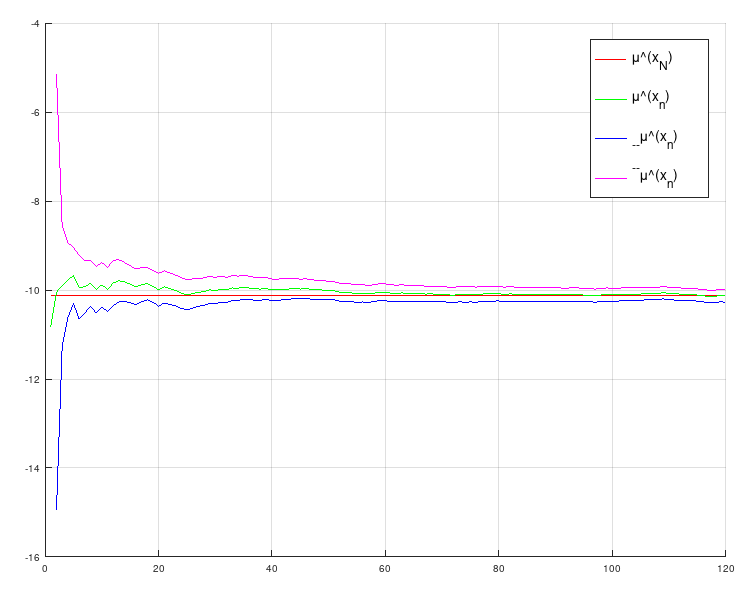
\includegraphics[scale=0.46]{assets/mu.png}
	\end{center}
	\caption{Оценка для мат. ожидания}
\end{figure}

\begin{figure}[H]
	\begin{center}
		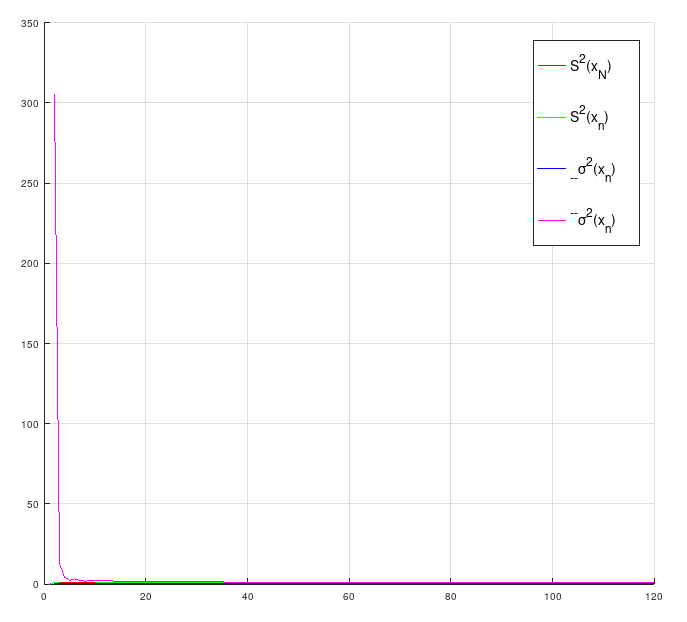
\includegraphics[scale=0.5]{assets/S2_1.png}
	\end{center}
	\caption{Оценка для дисперсии}
\end{figure}

\begin{figure}[H]
	\begin{center}
		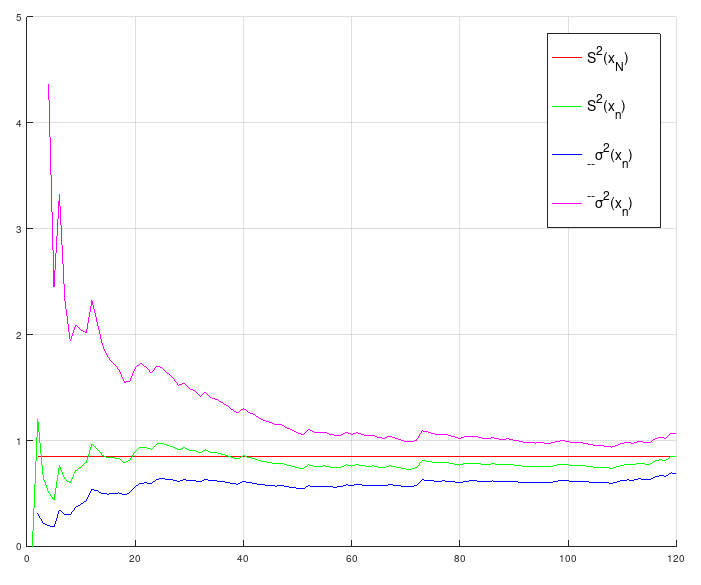
\includegraphics[scale=0.46]{assets/S2_2.png}
	\end{center}
	\caption{Оценка для дисперсии (график $\overline \sigma^2(\vec x_n)$ начинается с $n$ = 4)}
\end{figure}